% Options for packages loaded elsewhere
\PassOptionsToPackage{unicode}{hyperref}
\PassOptionsToPackage{hyphens}{url}
\PassOptionsToPackage{dvipsnames,svgnames,x11names}{xcolor}
%
\documentclass[
]{book}
\usepackage{amsmath,amssymb}
\usepackage{iftex}
\ifPDFTeX
  \usepackage[T1]{fontenc}
  \usepackage[utf8]{inputenc}
  \usepackage{textcomp} % provide euro and other symbols
\else % if luatex or xetex
  \usepackage{unicode-math} % this also loads fontspec
  \defaultfontfeatures{Scale=MatchLowercase}
  \defaultfontfeatures[\rmfamily]{Ligatures=TeX,Scale=1}
\fi
\usepackage{lmodern}
\ifPDFTeX\else
  % xetex/luatex font selection
\fi
% Use upquote if available, for straight quotes in verbatim environments
\IfFileExists{upquote.sty}{\usepackage{upquote}}{}
\IfFileExists{microtype.sty}{% use microtype if available
  \usepackage[]{microtype}
  \UseMicrotypeSet[protrusion]{basicmath} % disable protrusion for tt fonts
}{}
\makeatletter
\@ifundefined{KOMAClassName}{% if non-KOMA class
  \IfFileExists{parskip.sty}{%
    \usepackage{parskip}
  }{% else
    \setlength{\parindent}{0pt}
    \setlength{\parskip}{6pt plus 2pt minus 1pt}}
}{% if KOMA class
  \KOMAoptions{parskip=half}}
\makeatother
\usepackage{xcolor}
\usepackage[b5paper,tmargin=1.5cm,bmargin=1.5cm,lmargin=1.0cm,rmargin=1.0cm]{geometry}
\usepackage{color}
\usepackage{fancyvrb}
\newcommand{\VerbBar}{|}
\newcommand{\VERB}{\Verb[commandchars=\\\{\}]}
\DefineVerbatimEnvironment{Highlighting}{Verbatim}{commandchars=\\\{\}}
% Add ',fontsize=\small' for more characters per line
\usepackage{framed}
\definecolor{shadecolor}{RGB}{248,248,248}
\newenvironment{Shaded}{\begin{snugshade}}{\end{snugshade}}
\newcommand{\AlertTok}[1]{\textcolor[rgb]{0.94,0.16,0.16}{#1}}
\newcommand{\AnnotationTok}[1]{\textcolor[rgb]{0.56,0.35,0.01}{\textbf{\textit{#1}}}}
\newcommand{\AttributeTok}[1]{\textcolor[rgb]{0.13,0.29,0.53}{#1}}
\newcommand{\BaseNTok}[1]{\textcolor[rgb]{0.00,0.00,0.81}{#1}}
\newcommand{\BuiltInTok}[1]{#1}
\newcommand{\CharTok}[1]{\textcolor[rgb]{0.31,0.60,0.02}{#1}}
\newcommand{\CommentTok}[1]{\textcolor[rgb]{0.56,0.35,0.01}{\textit{#1}}}
\newcommand{\CommentVarTok}[1]{\textcolor[rgb]{0.56,0.35,0.01}{\textbf{\textit{#1}}}}
\newcommand{\ConstantTok}[1]{\textcolor[rgb]{0.56,0.35,0.01}{#1}}
\newcommand{\ControlFlowTok}[1]{\textcolor[rgb]{0.13,0.29,0.53}{\textbf{#1}}}
\newcommand{\DataTypeTok}[1]{\textcolor[rgb]{0.13,0.29,0.53}{#1}}
\newcommand{\DecValTok}[1]{\textcolor[rgb]{0.00,0.00,0.81}{#1}}
\newcommand{\DocumentationTok}[1]{\textcolor[rgb]{0.56,0.35,0.01}{\textbf{\textit{#1}}}}
\newcommand{\ErrorTok}[1]{\textcolor[rgb]{0.64,0.00,0.00}{\textbf{#1}}}
\newcommand{\ExtensionTok}[1]{#1}
\newcommand{\FloatTok}[1]{\textcolor[rgb]{0.00,0.00,0.81}{#1}}
\newcommand{\FunctionTok}[1]{\textcolor[rgb]{0.13,0.29,0.53}{\textbf{#1}}}
\newcommand{\ImportTok}[1]{#1}
\newcommand{\InformationTok}[1]{\textcolor[rgb]{0.56,0.35,0.01}{\textbf{\textit{#1}}}}
\newcommand{\KeywordTok}[1]{\textcolor[rgb]{0.13,0.29,0.53}{\textbf{#1}}}
\newcommand{\NormalTok}[1]{#1}
\newcommand{\OperatorTok}[1]{\textcolor[rgb]{0.81,0.36,0.00}{\textbf{#1}}}
\newcommand{\OtherTok}[1]{\textcolor[rgb]{0.56,0.35,0.01}{#1}}
\newcommand{\PreprocessorTok}[1]{\textcolor[rgb]{0.56,0.35,0.01}{\textit{#1}}}
\newcommand{\RegionMarkerTok}[1]{#1}
\newcommand{\SpecialCharTok}[1]{\textcolor[rgb]{0.81,0.36,0.00}{\textbf{#1}}}
\newcommand{\SpecialStringTok}[1]{\textcolor[rgb]{0.31,0.60,0.02}{#1}}
\newcommand{\StringTok}[1]{\textcolor[rgb]{0.31,0.60,0.02}{#1}}
\newcommand{\VariableTok}[1]{\textcolor[rgb]{0.00,0.00,0.00}{#1}}
\newcommand{\VerbatimStringTok}[1]{\textcolor[rgb]{0.31,0.60,0.02}{#1}}
\newcommand{\WarningTok}[1]{\textcolor[rgb]{0.56,0.35,0.01}{\textbf{\textit{#1}}}}
\usepackage{longtable,booktabs,array}
\usepackage{calc} % for calculating minipage widths
% Correct order of tables after \paragraph or \subparagraph
\usepackage{etoolbox}
\makeatletter
\patchcmd\longtable{\par}{\if@noskipsec\mbox{}\fi\par}{}{}
\makeatother
% Allow footnotes in longtable head/foot
\IfFileExists{footnotehyper.sty}{\usepackage{footnotehyper}}{\usepackage{footnote}}
\makesavenoteenv{longtable}
\usepackage{graphicx}
\makeatletter
\def\maxwidth{\ifdim\Gin@nat@width>\linewidth\linewidth\else\Gin@nat@width\fi}
\def\maxheight{\ifdim\Gin@nat@height>\textheight\textheight\else\Gin@nat@height\fi}
\makeatother
% Scale images if necessary, so that they will not overflow the page
% margins by default, and it is still possible to overwrite the defaults
% using explicit options in \includegraphics[width, height, ...]{}
\setkeys{Gin}{width=\maxwidth,height=\maxheight,keepaspectratio}
% Set default figure placement to htbp
\makeatletter
\def\fps@figure{htbp}
\makeatother
\setlength{\emergencystretch}{3em} % prevent overfull lines
\providecommand{\tightlist}{%
  \setlength{\itemsep}{0pt}\setlength{\parskip}{0pt}}
\setcounter{secnumdepth}{5}
\newlength{\cslhangindent}
\setlength{\cslhangindent}{1.5em}
\newlength{\csllabelwidth}
\setlength{\csllabelwidth}{3em}
\newlength{\cslentryspacingunit} % times entry-spacing
\setlength{\cslentryspacingunit}{\parskip}
\newenvironment{CSLReferences}[2] % #1 hanging-ident, #2 entry spacing
 {% don't indent paragraphs
  \setlength{\parindent}{0pt}
  % turn on hanging indent if param 1 is 1
  \ifodd #1
  \let\oldpar\par
  \def\par{\hangindent=\cslhangindent\oldpar}
  \fi
  % set entry spacing
  \setlength{\parskip}{#2\cslentryspacingunit}
 }%
 {}
\usepackage{calc}
\newcommand{\CSLBlock}[1]{#1\hfill\break}
\newcommand{\CSLLeftMargin}[1]{\parbox[t]{\csllabelwidth}{#1}}
\newcommand{\CSLRightInline}[1]{\parbox[t]{\linewidth - \csllabelwidth}{#1}\break}
\newcommand{\CSLIndent}[1]{\hspace{\cslhangindent}#1}
\usepackage{booktabs}
% \usepackage{fontspec} %這個可能原本文檔就已經有了,放入時候check一下
% \usepackage{CJKutf8}
% \usepackage[UTF8]{inputenc}
\usepackage{CJK}
% \usepackage{xeCJK}

%英文字體調整(有時候交中文文件可能有規定對應的英文字體)
% \setmainfont{Times New Roman}
% \setmainfont{Noto Sans}

%中文字體main跟mono都需要哦,最後面的SC是簡體中文,也可以改成TC,不過SC的破字會比較少
% \setCJKmainfont{NotoSansTC-Regular.otf}
% \setCJKmonofont{NotoSansTC-Regular.otf}

% \usepackage{bm}
\usepackage{amsmath,amssymb}
\usepackage{hyperref}
\hypersetup{
    colorlinks=true,
    linkcolor=blue,
    filecolor=magenta,      
    urlcolor=cyan
}

% to wrap the text inside the margins of the PDF document when using code chunks in bookdown
\usepackage{fvextra}
\DefineVerbatimEnvironment{Highlighting}{Verbatim}{breaklines,commandchars=\\\{\}}

% \usepackage[backend=bibtex]{biblatex}
% \usepackage[backend=biber]{biblatex}
% \usepackage[]{biblatex}
% \DeclarePrintbibliographyDefaults{heading=bibintoc}

% \let\oldpb\printbibliography
% \renewcommand{\printbibliography}{\oldpb[heading=bibintoc]}

\usepackage{pgfplots}
\pgfplotsset{compat=1.15}
\usepackage{mathrsfs}
\usetikzlibrary{arrows}
% \pagestyle{empty}
% \newcommand{\degre}{\ensuremath{^\circ}}

\usepackage[all]{xy}

% LaTeX Error: Too deeply nested
% https://stackoverflow.com/questions/57945414/too-deeply-nested-at-just-fourth-nesting-level-using-pandoc-with-markdown
\usepackage{enumitem}
\setlistdepth{20}
\renewlist{itemize}{itemize}{20}
\renewlist{enumerate}{enumerate}{20}
\setlist[itemize]{label=$\cdot$}
\setlist[itemize,1]{label=\textbullet}
\setlist[itemize,2]{label=--}
\setlist[itemize,3]{label=*}
\ifLuaTeX
  \usepackage{selnolig}  % disable illegal ligatures
\fi
\IfFileExists{bookmark.sty}{\usepackage{bookmark}}{\usepackage{hyperref}}
\IfFileExists{xurl.sty}{\usepackage{xurl}}{} % add URL line breaks if available
\urlstyle{same}
\hypersetup{
  pdftitle={math},
  pdfauthor={Joey Yu Hsu},
  colorlinks=true,
  linkcolor={Maroon},
  filecolor={Maroon},
  citecolor={Blue},
  urlcolor={Blue},
  pdfcreator={LaTeX via pandoc}}

\title{math}
\author{Joey Yu Hsu}
\date{2024-01-31}

\usepackage{amsthm}
\newtheorem{theorem}{Theorem}[chapter]
\newtheorem{lemma}{Lemma}[chapter]
\newtheorem{corollary}{Corollary}[chapter]
\newtheorem{proposition}{Proposition}[chapter]
\newtheorem{conjecture}{Conjecture}[chapter]
\theoremstyle{definition}
\newtheorem{definition}{Definition}[chapter]
\theoremstyle{definition}
\newtheorem{example}{Example}[chapter]
\theoremstyle{definition}
\newtheorem{exercise}{Exercise}[chapter]
\theoremstyle{definition}
\newtheorem{hypothesis}{Hypothesis}[chapter]
\theoremstyle{remark}
\newtheorem*{remark}{Remark}
\newtheorem*{solution}{Solution}
\begin{document}
\maketitle

{
\hypersetup{linkcolor=}
\setcounter{tocdepth}{1}
\tableofcontents
}
\hypertarget{index}{%
\chapter*{index}\label{index}}
\addcontentsline{toc}{chapter}{index}

math on bookdown started on 2024/01/28

script\textsuperscript{superscript}\textsubscript{subscript}

\hypertarget{part-ordered-by-discipline}{%
\part{ordered by discipline}\label{part-ordered-by-discipline}}

\protect\hyperlink{nice-label}{math}

\hypertarget{test-cross-link}{%
\chapter{test cross-link}\label{test-cross-link}}

\hypertarget{link-and-reference}{%
\section{link and reference}\label{link-and-reference}}

\ref{nice-label}

\protect\hyperlink{partition}{link to partition}

\protect\hyperlink{partition}{partition} {[}\#partition{]} (\ref{partition}) @ref(\#partition)

\protect\hyperlink{equivalence-class}{equivalence class} {[}\#equivalence class{]} (@ref(equivalence class)) @ref(\#equivalence class)

{[}equivalence-class{]} {[}\#equivalence-class{]} (\ref{equivalence-class}) @ref(\#equivalence-class)

{[}equivalence-class.html{]} {[}equivalence-class.html\#equivalence-class{]} (@ref(equivalence-class.html)) @ref(equivalence-class.html\#equivalence-class)

\protect\hyperlink{equivalence-relation}{equivalence relation} {[}\#equivalence relation{]} (@ref(equivalence relation)) @ref(\#equivalence relation)

{[}equivalence-relation{]} {[}\#equivalence-relation{]} (\ref{equivalence-relation}) @ref(\#equivalence-relation)

{[}equivalence-relation.html{]} {[}equivalence-relation.html\#equivalence-relation{]} (@ref(equivalence-relation.html)) @ref(equivalence-relation.html\#equivalence-relation)

\hypertarget{footnote}{%
\section{footnote}\label{footnote}}

noun\footnote{This is a footnote.}

\hypertarget{citation}{%
\section{citation}\label{citation}}

\url{https://stackoverflow.com/questions/48965247/use-csl-file-for-pdf-output-in-bookdown/49145699\#49145699}

citation 1\textsuperscript{\protect\hyperlink{ref-noauthor_bookdown_2019}{1}} citation 2\textsuperscript{\protect\hyperlink{ref-noauthor_bookdown_2019}{1}}

citation 3\textsuperscript{\protect\hyperlink{ref-ccjou2009}{2}} citation 4\textsuperscript{\protect\hyperlink{ref-ccjou2009}{2}}

\hypertarget{bookdown-environment-for-definition-theorem-proof}{%
\section{bookdown environment for definition, theorem, proof}\label{bookdown-environment-for-definition-theorem-proof}}

\url{https://bookdown.org/yihui/rmarkdown/bookdown-markdown.html}

\begin{theorem}[Theorem Name]
\protect\hypertarget{thm:label}{}\label{thm:label}Here is my theorem.
\end{theorem}

\begin{proof}[Proof Name]
Here is my proof.
\end{proof}

\begin{theorem}[Pythagorean theorem]
\protect\hypertarget{thm:pyth}{}\label{thm:pyth}For a right triangle, if \(c\) denotes the length of the hypotenuse
and \(a\) and \(b\) denote the lengths of the other two sides, we have

\[a^2 + b^2 = c^2\]
\end{theorem}

\begin{definition}[Definition Name]
\protect\hypertarget{def:unnamed-chunk-2}{}\label{def:unnamed-chunk-2}Here is my definition.
\end{definition}

\hypertarget{nice-label}{%
\chapter{math}\label{nice-label}}

\protect\hyperlink{equivalence-relation}{equivalence relation} \ref{equivalence-relation}

\protect\hyperlink{equivalence-class}{equivalence class} \ref{equivalence-class}

\protect\hyperlink{partition}{partition} \ref{partition}

\hypertarget{equivalence-relation}{%
\chapter*{equivalence relation}\label{equivalence-relation}}
\addcontentsline{toc}{chapter}{equivalence relation}

\begin{CJK}{UTF8}{bsmi}等價關係 equivalence relation \label{def:equivalence-relation}
\end{CJK}
\begin{CJK}{UTF8}{bsmi}
\begin{align*}
 & R\text{ is an equivalence relation over }A\times B\\
\Leftrightarrow & \begin{cases}
R=\sim=\left\{ \left\langle x,y\right\rangle \middle|x\sim y\right\} \subseteq A\times B & \left(\text{e}\right)\text{equivalence 等價}\\
\vdots & \vdots
\end{cases}\\
\Leftrightarrow & \begin{cases}
R=\left\{ \left\langle x,y\right\rangle \middle|xRy\right\} \subseteq A\times B & \left(R\right)\text{relation}\\
\forall\left\langle x,y\right\rangle \in R\left(xRx\right) & \left(r\right)\text{reflexive}\\
\forall\left\langle x,y\right\rangle \in R\left(xRy\Rightarrow yRx\right) & \left(s\right)\text{symmetric}\\
\forall\left\langle x,y\right\rangle ,\left\langle y,z\right\rangle \in R\left(\begin{cases}
xRy\\
yRz
\end{cases}\Rightarrow xRz\right) & \left(t\right)\text{transitive}
\end{cases}\Leftrightarrow\begin{cases}
R=\left\{ \left\langle x,y\right\rangle \middle|xRy\right\} \subseteq A\times B & \text{關係}\\
\forall\left\langle x,y\right\rangle \in R\left(\left\langle x,x\right\rangle \in R\right) & \text{自反}\\
\forall\left\langle x,y\right\rangle \in R\left(\left\langle y,x\right\rangle \in R\right) & \text{對稱}\\
\forall\left\langle x,y\right\rangle ,\left\langle y,z\right\rangle \in R\left(\left\langle x,z\right\rangle \in R\right) & \text{遞移}
\end{cases}
\end{align*}
\end{CJK}

\hypertarget{equivalence-class}{%
\chapter*{equivalence class}\label{equivalence-class}}
\addcontentsline{toc}{chapter}{equivalence class}

\begin{align*}
 & C\text{ is an equivalence class of }a\text{ on }A\\
\Leftrightarrow & \left[a\right]_{\sim}=C=\left\{ x\middle|\begin{cases}
a\in A\\
x\in A\\
x\sim a\\
\sim\text{ is an equivalence relation over }A\times A=A^{2}
\end{cases}\right\} \subseteq A\ne\emptyset\\
\Leftrightarrow & \left[a\right]=\left[a\right]_{\sim}=\left\{ x\middle|\begin{cases}
a\in A\\
x\in A\\
x\sim a\\
\sim\text{ is an equivalence relation on }A
\end{cases}\right\} \subseteq A\ne\emptyset\\
\Rightarrow & \left[a\right]_{\sim}=\left\{ x\middle|x\sim a\right\} \subseteq A\ne\emptyset
\end{align*}

where \protect\hyperlink{equivalence-relation}{equivalence relation} \ref{equivalence-relation}

\hypertarget{physics}{%
\chapter{physics}\label{physics}}

\hypertarget{partition}{%
\chapter*{partition}\label{partition}}
\addcontentsline{toc}{chapter}{partition}

\begin{align*}
 & \left\{ A_{i}\right\} _{i\in I}=\left\{ A_{i}\middle|i\in I\right\} \text{ is a partition of a set }A\\
\Leftrightarrow & \begin{cases}
\forall i\in I\left(A_{i}\ne\emptyset\right)\\
A=\bigcup\limits _{i\in I}A_{i}\\
\forall i,j\in I\left(i\ne j\Rightarrow A_{i}\cap A_{j}=\emptyset\right)
\end{cases}
\end{align*}

\url{https://proofwiki.org/wiki/Definition:Set_Partition}

\hypertarget{plot}{%
\chapter{plot}\label{plot}}

\hypertarget{tikzpgfplot}{%
\chapter*{TiKZ/PgfPlot}\label{tikzpgfplot}}
\addcontentsline{toc}{chapter}{TiKZ/PgfPlot}

\begin{figure}
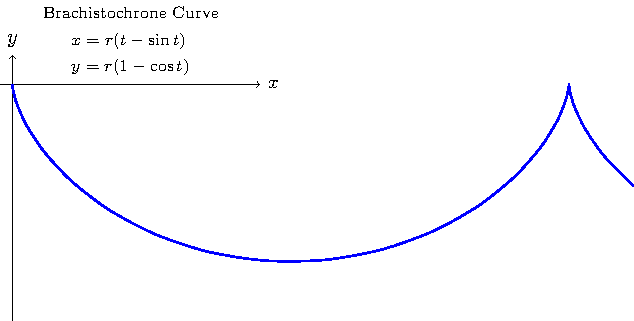
\includegraphics[width=0.9\linewidth]{202401260003-plot_files/figure-latex/unnamed-chunk-3-1} \caption{Brachistochrone Curve}\label{fig:unnamed-chunk-3}
\end{figure}

\begin{figure}
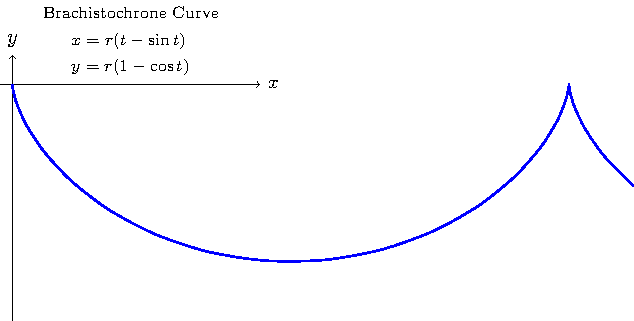
\includegraphics[width=0.9\linewidth]{202401260003-plot_files/figure-latex/unnamed-chunk-4-1} \caption{Brachistochrone Curve}\label{fig:unnamed-chunk-4}
\end{figure}

\hypertarget{xy-pic}{%
\chapter*{xy-pic}\label{xy-pic}}
\addcontentsline{toc}{chapter}{xy-pic}

\url{https://bookdown.org/yihui/rmarkdown-cookbook/install-latex-pkgs.html}

\texttt{tinytex::install\_tinytex()}

the following xymatrix from LaTeX package xy for xy-pic is not shown or rendered in HTML:

\texttt{\$\textbackslash{}LaTeX\$} can only be used in HTML, not PDF

\xymatrix{U\ar[ddr]_{\psi}\ar[drr]^{\varphi}\ar[dr]|-{(x,y)}\\
 & X\times_{Z}Y\ar[d]^{q}\ar[r]_{p} & X\ar[d]_{f}\\
 & Y\ar[r]^{g} & Z
}

\[
\xymatrix{U\ar[ddr]_{\psi}\ar[drr]^{\varphi}\ar[dr]|-{(x,y)}\\
 & X\times_{Z}Y\ar[d]^{q}\ar[r]_{p} & X\ar[d]_{f}\\
 & Y\ar[r]^{g} & Z
}
\]

\hypertarget{part-ordered-by-date}{%
\part{ordered by date}\label{part-ordered-by-date}}

\hypertarget{ordered-by-date}{%
\chapter{ordered by date}\label{ordered-by-date}}

\hypertarget{partition-1}{%
\chapter*{partition}\label{partition-1}}
\addcontentsline{toc}{chapter}{partition}

\begin{align*}
 & \left\{ A_{i}\right\} _{i\in I}=\left\{ A_{i}\middle|i\in I\right\} \text{ is a partition of a set }A\\
\Leftrightarrow & \begin{cases}
\forall i\in I\left(A_{i}\ne\emptyset\right)\\
A=\bigcup\limits _{i\in I}A_{i}\\
\forall i,j\in I\left(i\ne j\Rightarrow A_{i}\cap A_{j}=\emptyset\right)
\end{cases}
\end{align*}

\url{https://proofwiki.org/wiki/Definition:Set_Partition}

\hypertarget{section}{%
\chapter*{202401281000}\label{section}}
\addcontentsline{toc}{chapter}{202401281000}

\hypertarget{equivalence-class-1}{%
\chapter*{equivalence class}\label{equivalence-class-1}}
\addcontentsline{toc}{chapter}{equivalence class}

\begin{align*}
 & C\text{ is an equivalence class of }a\text{ on }A\\
\Leftrightarrow & \left[a\right]_{\sim}=C=\left\{ x\middle|\begin{cases}
a\in A\\
x\in A\\
x\sim a\\
\sim\text{ is an equivalence relation over }A\times A=A^{2}
\end{cases}\right\} \subseteq A\ne\emptyset\\
\Leftrightarrow & \left[a\right]=\left[a\right]_{\sim}=\left\{ x\middle|\begin{cases}
a\in A\\
x\in A\\
x\sim a\\
\sim\text{ is an equivalence relation on }A
\end{cases}\right\} \subseteq A\ne\emptyset\\
\Rightarrow & \left[a\right]_{\sim}=\left\{ x\middle|x\sim a\right\} \subseteq A\ne\emptyset
\end{align*}

where \protect\hyperlink{equivalence-relation}{equivalence relation} \ref{equivalence-relation}

\hypertarget{equivalence-relation-1}{%
\chapter*{equivalence relation}\label{equivalence-relation-1}}
\addcontentsline{toc}{chapter}{equivalence relation}

\begin{CJK}{UTF8}{bsmi}等價關係 equivalence relation \label{def:equivalence-relation}
\end{CJK}
\begin{CJK}{UTF8}{bsmi}
\begin{align*}
 & R\text{ is an equivalence relation over }A\times B\\
\Leftrightarrow & \begin{cases}
R=\sim=\left\{ \left\langle x,y\right\rangle \middle|x\sim y\right\} \subseteq A\times B & \left(\text{e}\right)\text{equivalence 等價}\\
\vdots & \vdots
\end{cases}\\
\Leftrightarrow & \begin{cases}
R=\left\{ \left\langle x,y\right\rangle \middle|xRy\right\} \subseteq A\times B & \left(R\right)\text{relation}\\
\forall\left\langle x,y\right\rangle \in R\left(xRx\right) & \left(r\right)\text{reflexive}\\
\forall\left\langle x,y\right\rangle \in R\left(xRy\Rightarrow yRx\right) & \left(s\right)\text{symmetric}\\
\forall\left\langle x,y\right\rangle ,\left\langle y,z\right\rangle \in R\left(\begin{cases}
xRy\\
yRz
\end{cases}\Rightarrow xRz\right) & \left(t\right)\text{transitive}
\end{cases}\Leftrightarrow\begin{cases}
R=\left\{ \left\langle x,y\right\rangle \middle|xRy\right\} \subseteq A\times B & \text{關係}\\
\forall\left\langle x,y\right\rangle \in R\left(\left\langle x,x\right\rangle \in R\right) & \text{自反}\\
\forall\left\langle x,y\right\rangle \in R\left(\left\langle y,x\right\rangle \in R\right) & \text{對稱}\\
\forall\left\langle x,y\right\rangle ,\left\langle y,z\right\rangle \in R\left(\left\langle x,z\right\rangle \in R\right) & \text{遞移}
\end{cases}
\end{align*}
\end{CJK}

\hypertarget{python}{%
\chapter{Python}\label{python}}

\url{https://bookdown.org/yihui/rmarkdown/language-engines.html}

\begin{Shaded}
\begin{Highlighting}[]
\FunctionTok{names}\NormalTok{(knitr}\SpecialCharTok{::}\NormalTok{knit\_engines}\SpecialCharTok{$}\FunctionTok{get}\NormalTok{())}
\end{Highlighting}
\end{Shaded}

\begin{verbatim}
##  [1] "awk"         "bash"        "coffee"      "gawk"        "groovy"     
##  [6] "haskell"     "lein"        "mysql"       "node"        "octave"     
## [11] "perl"        "php"         "psql"        "Rscript"     "ruby"       
## [16] "sas"         "scala"       "sed"         "sh"          "stata"      
## [21] "zsh"         "asis"        "asy"         "block"       "block2"     
## [26] "bslib"       "c"           "cat"         "cc"          "comment"    
## [31] "css"         "ditaa"       "dot"         "embed"       "eviews"     
## [36] "exec"        "fortran"     "fortran95"   "go"          "highlight"  
## [41] "js"          "julia"       "python"      "R"           "Rcpp"       
## [46] "sass"        "scss"        "sql"         "stan"        "targets"    
## [51] "tikz"        "verbatim"    "theorem"     "lemma"       "corollary"  
## [56] "proposition" "conjecture"  "definition"  "example"     "exercise"   
## [61] "hypothesis"  "proof"       "remark"      "solution"    "glue"       
## [66] "glue_sql"    "gluesql"
\end{verbatim}

\url{https://rstudio.github.io/reticulate/articles/python_packages.html}

\begin{Shaded}
\begin{Highlighting}[]
\NormalTok{x }\OperatorTok{=} \StringTok{\textquotesingle{}hello, python world!\textquotesingle{}}
\BuiltInTok{print}\NormalTok{(x.split(}\StringTok{\textquotesingle{} \textquotesingle{}}\NormalTok{))}
\end{Highlighting}
\end{Shaded}

\begin{verbatim}
## ['hello,', 'python', 'world!']
\end{verbatim}

\begin{Shaded}
\begin{Highlighting}[]
\FunctionTok{library}\NormalTok{(reticulate)}
\end{Highlighting}
\end{Shaded}

\begin{verbatim}
## Warning: package 'reticulate' was built under R version 4.2.3
\end{verbatim}

\begin{Shaded}
\begin{Highlighting}[]
\FunctionTok{virtualenv\_python}\NormalTok{()}
\end{Highlighting}
\end{Shaded}

\begin{verbatim}
## [1] "D:/Users/115381/Documents/.virtualenvs/r-reticulate/Scripts/python.exe"
\end{verbatim}

\begin{Shaded}
\begin{Highlighting}[]
\FunctionTok{library}\NormalTok{(reticulate)}
\FunctionTok{conda\_list}\NormalTok{()}
\end{Highlighting}
\end{Shaded}

\begin{verbatim}
##                name                                            python
## 1              base                          D:\\Anaconda3/python.exe
## 2          fiftyone          D:\\Anaconda3\\envs\\fiftyone/python.exe
## 3             keras             D:\\Anaconda3\\envs\\keras/python.exe
## 4           labelme           D:\\Anaconda3\\envs\\labelme/python.exe
## 5             manim             D:\\Anaconda3\\envs\\manim/python.exe
## 6            mmyolo            D:\\Anaconda3\\envs\\mmyolo/python.exe
## 7 rsconnect-jupyter D:\\Anaconda3\\envs\\rsconnect-jupyter/python.exe
## 8           sandbox           D:\\Anaconda3\\envs\\sandbox/python.exe
## 9       sandbox-3.9       D:\\Anaconda3\\envs\\sandbox-3.9/python.exe
\end{verbatim}

\url{https://rstudio.github.io/reticulate/reference/install_python.html}

\begin{Shaded}
\begin{Highlighting}[]
\FunctionTok{library}\NormalTok{(reticulate)}
\NormalTok{version }\OtherTok{\textless{}{-}} \StringTok{"3.9.12"}
\CommentTok{\# install\_python(version)}

\CommentTok{\# create a new environment }
\CommentTok{\# virtualenv\_create("r{-}reticulate", version = version)}

\CommentTok{\# use\_virtualenv("r{-}reticulate")}

\CommentTok{\# install MatPlotLib}
\CommentTok{\# virtualenv\_install("r{-}reticulate", "matplotlib")}

\CommentTok{\# import MatPlotLib (it will be automatically discovered in "r{-}reticulate")}
\NormalTok{matplotlib }\OtherTok{\textless{}{-}} \FunctionTok{import}\NormalTok{(}\StringTok{"matplotlib"}\NormalTok{)}
\end{Highlighting}
\end{Shaded}

\begin{Shaded}
\begin{Highlighting}[]
\FunctionTok{library}\NormalTok{(reticulate)}
\FunctionTok{virtualenv\_list}\NormalTok{()}
\end{Highlighting}
\end{Shaded}

\begin{verbatim}
## [1] "r-reticulate"
\end{verbatim}

\begin{Shaded}
\begin{Highlighting}[]
\CommentTok{\# library(reticulate)}
\CommentTok{\# use\_virtualenv("r{-}reticulate")}
\CommentTok{\# matplotlib \textless{}{-} import("matplotlib")}
\CommentTok{\# matplotlib$use("Agg", force = TRUE)}
\end{Highlighting}
\end{Shaded}

\begin{Shaded}
\begin{Highlighting}[]
\ImportTok{import}\NormalTok{ matplotlib.pyplot }\ImportTok{as}\NormalTok{ plt}
\NormalTok{plt.plot([}\DecValTok{0}\NormalTok{, }\DecValTok{2}\NormalTok{, }\DecValTok{1}\NormalTok{, }\DecValTok{4}\NormalTok{])}
\NormalTok{plt.show()}
\end{Highlighting}
\end{Shaded}

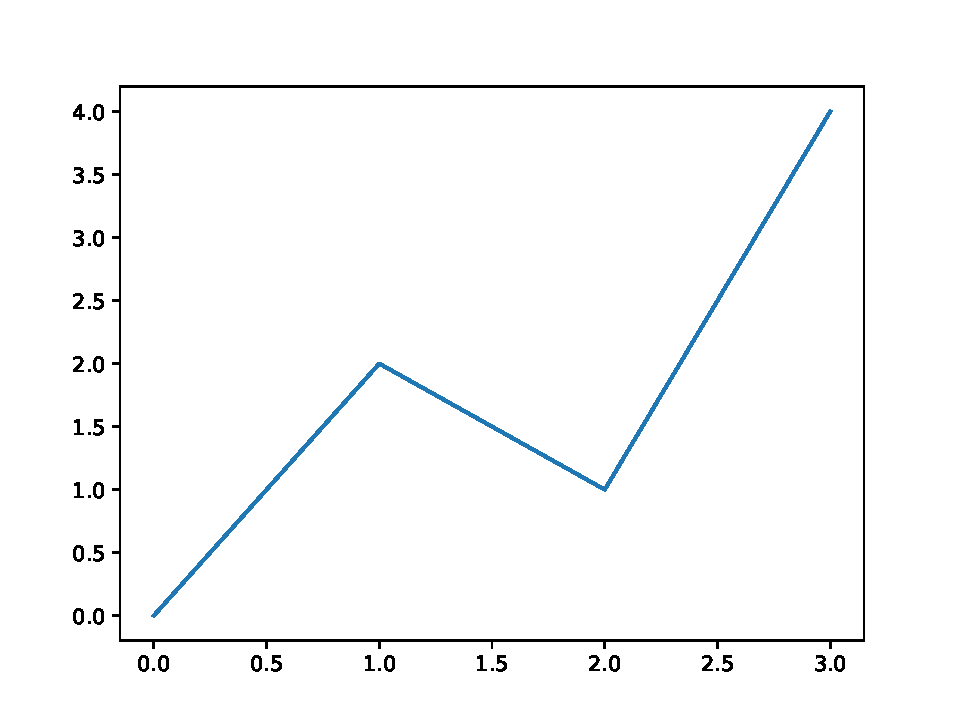
\includegraphics{202401292317-Python_files/figure-latex/unnamed-chunk-8-1.pdf}

\hypertarget{tikzpgfplot-1}{%
\chapter*{TiKZ/PgfPlot}\label{tikzpgfplot-1}}
\addcontentsline{toc}{chapter}{TiKZ/PgfPlot}

\begin{figure}
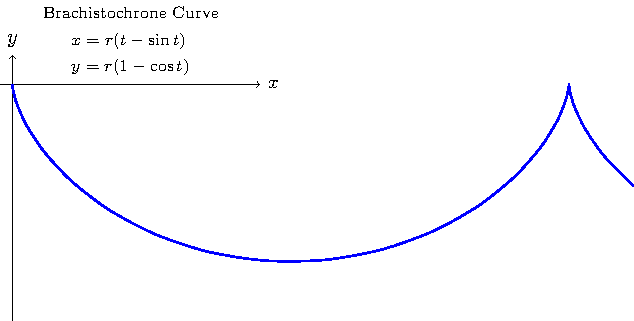
\includegraphics[width=0.9\linewidth]{202401311000-TiKZ-PgfPlot_files/figure-latex/unnamed-chunk-1-1} \caption{Brachistochrone Curve}\label{fig:unnamed-chunk-1}
\end{figure}

\begin{figure}
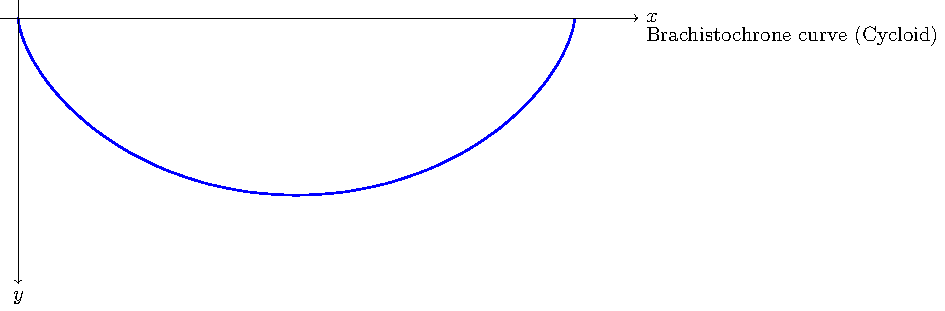
\includegraphics[width=0.9\linewidth]{202401311000-TiKZ-PgfPlot_files/figure-latex/unnamed-chunk-2-1} \caption{Brachistochrone Curve}\label{fig:unnamed-chunk-2}
\end{figure}

\hypertarget{xy-pic-1}{%
\chapter*{xy-pic}\label{xy-pic-1}}
\addcontentsline{toc}{chapter}{xy-pic}

\url{https://bookdown.org/yihui/rmarkdown-cookbook/install-latex-pkgs.html}

\texttt{tinytex::install\_tinytex()}

the following xymatrix from LaTeX package xy for xy-pic is not shown or rendered in HTML:

\texttt{\$\textbackslash{}LaTeX\$} can only be used in HTML, not PDF

\xymatrix{U\ar[ddr]_{\psi}\ar[drr]^{\varphi}\ar[dr]|-{(x,y)}\\
 & X\times_{Z}Y\ar[d]^{q}\ar[r]_{p} & X\ar[d]_{f}\\
 & Y\ar[r]^{g} & Z
}

\[
\xymatrix{U\ar[ddr]_{\psi}\ar[drr]^{\varphi}\ar[dr]|-{(x,y)}\\
 & X\times_{Z}Y\ar[d]^{q}\ar[r]_{p} & X\ar[d]_{f}\\
 & Y\ar[r]^{g} & Z
}
\]

\hypertarget{references}{%
\chapter*{references}\label{references}}
\addcontentsline{toc}{chapter}{references}
\begin{CJK}{UTF8}{bsmi}
\hypertarget{refs}{}
\begin{CSLReferences}{0}{0}
\leavevmode\vadjust pre{\hypertarget{ref-noauthor_bookdown_2019}{}}%
\CSLLeftMargin{1. }%
\CSLRightInline{\href{https://community.rstudio.com/t/bookdown-books-on-the-web-downloading-and-converting-to-pdf/30268}{Bookdown books on the web: Downloading and converting to pdf - {R} {Markdown}}. \emph{Posit Community} (2019).}

\leavevmode\vadjust pre{\hypertarget{ref-ccjou2009}{}}%
\CSLLeftMargin{2. }%
\CSLRightInline{ccjou. \href{https://ccjou.wordpress.com/2009/10/21/\%e4\%ba\%8c\%e6\%ac\%a1\%e5\%9e\%8b\%e8\%88\%87\%e6\%ad\%a3\%e5\%ae\%9a\%e7\%9f\%a9\%e9\%99\%a3/}{二次型與正定矩陣}. (2009).}

\end{CSLReferences}
\end{CJK}

\end{document}
